\section{The Forward Translation}\label{sec:forward-translation}
\glsreset{teo}
The translation process starts with semantic \LaTeX{} expressions. These expressions get analyzed and parsed by the \gls{mlp}, which produces a \gls{mlp-pt} of the input expression with additional information about each symbol. An abstract translator class analyzes each node and delegates them to specialized subtranslators. In this process an object called \gls{teo} is build. This \gls{teo} is needed to rebuild a string representation of the mathematical expression given by the \gls{mlp-pt}.

The overall forward translation process is explained in figure~\ref{fig:forward-trans}. All translation patterns and related information are stored in the DLMF/DRMF tables. These tables are converted by the \verb|lexicon-creator.jar| to the \verb|DLMF-macros-lexicon.txt| lexicon file. Together with the \verb|global-lexicon.txt| file, the \gls{mlp-pt} will be created by the \gls{mlp}. The \verb|latex-converter.jar| takes a string representation of a semantic \LaTeX{} expression and uses the \gls{mlp} as well as our \verb|Translator| to create an appropriate string representation for a specified \gls{cas}. The following \cref{subsec:analyze-mlp,subsec:delegation,subsec:translated-expr,subsec:add-info} will focus on the \verb|Translator|.

\begin{figure}[ht]
	\vspace{-10pt}
	\centering
	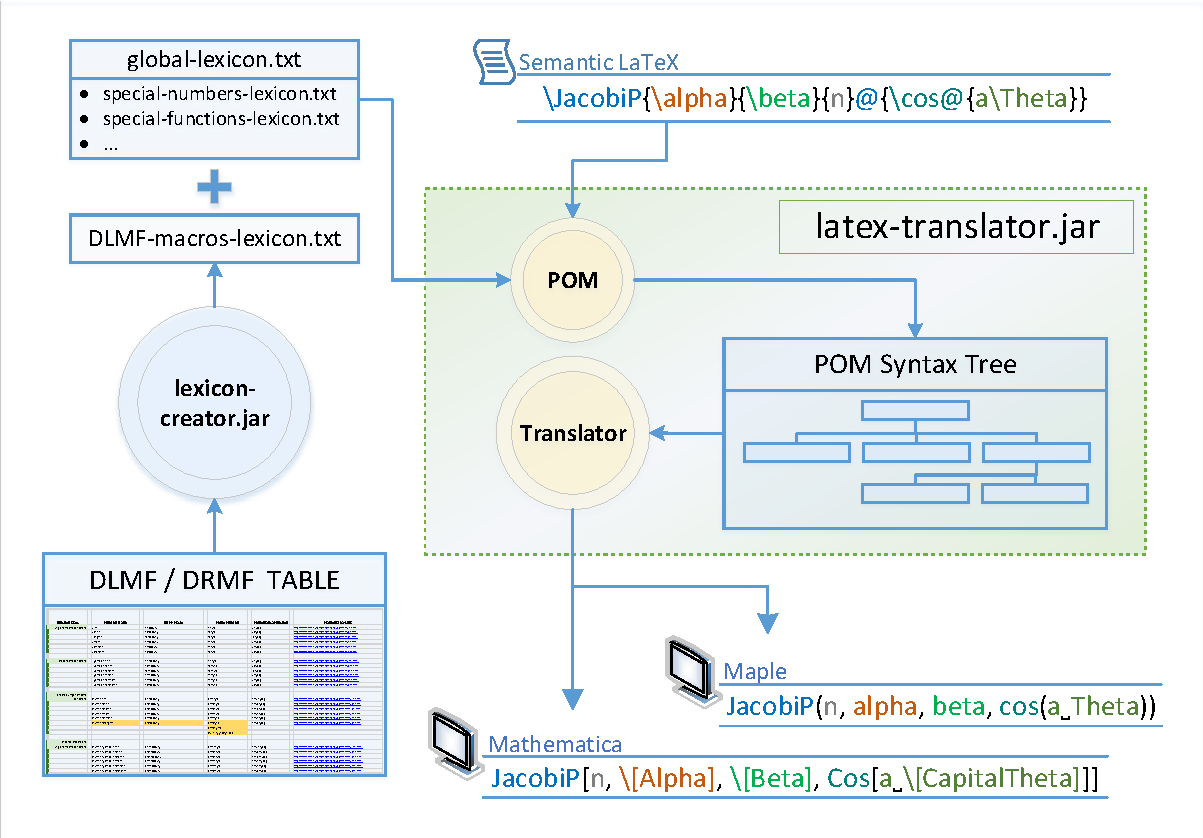
\includegraphics[clip, trim=0.2cm 0.2cm 0.2cm 0.2cm, scale=0.72]{ForwardTranslationProcess.pdf}
	\caption{Process diagram of a forward translation process. The MLP generates the PT based on lexicon and JSON files. The PT will be translated to different CAS.}
	\label{fig:forward-trans}
	\vspace{-10pt}
\end{figure}

\subsection{Analyzing the MLP-Parse Tree}\label{subsec:analyze-mlp}
The main task is to analyze the \gls{mlp-pt}. Remember that the \gls{mlp-pt} is different to expression trees as described in section~\ref{subsec:pom-mlp}.

Since the \gls{bnf} does not define rules for semantic macros, each argument of the semantic macro and each $@$ symbol are following siblings of the semantic macro node. That is the reason, why we stored the number of parameters, variables and $@$ symbols in the lexicon files. Otherwise, the translator could not find the end of a semantic macro in the \gls{mlp-pt}.

Figure~\ref{fig:syntax-tree-usecase} visualizes the \gls{mlp-pt} of the Jacobi polynomial example from table~\ref{tab:JacobiP-usecase}. Because of these differences to expression trees, a backward conversion of the \gls{mlp-pt} to a string representation can be difficult, especially for finding necessary or unnecessary parentheses. Therefore we create the \gls{teo}. Of course, the \gls{teo} is deeply incorporated into the translation process, but in this subsection we will focus on the general idea and process of the translation. We will focus on the usage of \gls{teo} in subsection~\ref{subsec:translated-expr}.

\begin{figure}[ht]
	\centering
	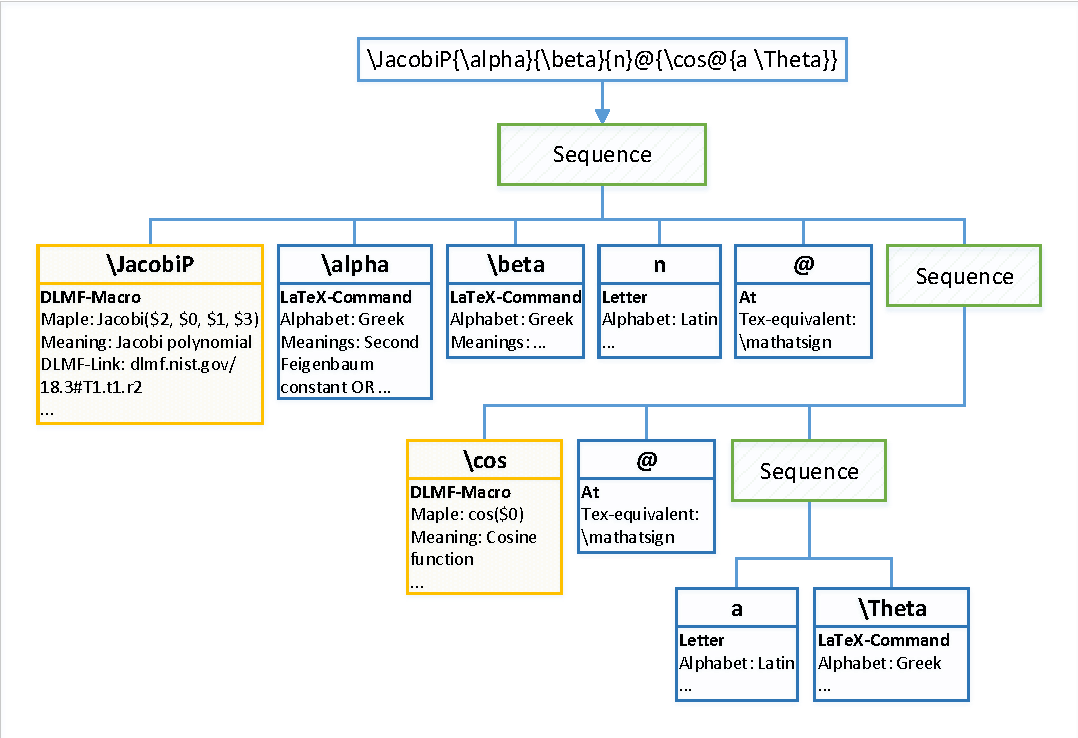
\includegraphics[clip, trim=0.2cm 0.2cm 0.2cm 0.2cm, scale=0.75]{SyntaxTreeUseCase.pdf}
	\caption{MLP-PT for a Jacobi polynomial using the DLMF/DRMF \LaTeX{} macro. Each leaf contains information from the lexicon files.}
	\label{fig:syntax-tree-usecase}
\end{figure}

The general idea of a translation of a \gls{mlp-pt} is a simple recursive algorithm, such as algorithm~\ref{alg:simple-translation}. Whenever the algorithm finds a leaf, it can translate this single term. If the node is not a leaf, it starts to translate all children of the node recursively. 

\begin{wrapfigure}{r}{0.5\textwidth}
\vspace{-20pt}
\begin{minipage}{0.5\textwidth}
\begin{algorithm}[H]
\caption{Simple translation algorithm for the MLP-Parse Tree}\label{alg:simple-translation}
	\begin{algorithmic}[1]
	\Require Root $r$ of the parse tree $T$
	\Procedure{translate}{$r$}
	\If{$r$ is leaf}
		\State {\scriptsize TRANSLATE\_LEAF}($r$);
	\Else
		\ForAll{children $v_n$ of $r$}
			\State {\scriptsize TRANSLATE}($v_n$);
		\EndFor
	\EndIf
	\EndProcedure
	\end{algorithmic}
\end{algorithm}
\end{minipage}
\vspace{-14pt}
\end{wrapfigure}

But this approach is not completely feasible, because sometimes the algorithm needs to look ahead and check the following siblings for a valid translation, for example in case of a semantic macro with arguments (see figure~\ref{fig:syntax-tree-usecase}). Therefore, the {\footnotesize \verb|TRANSLATE_LEAF|} function also needs to know the following siblings of the current node. To avoid multiple translations of the same node, a list representation would be a better solution. Algorithm~\ref{alg:translation} explains an abstract version of the final algorithm for our translation tool. 

If the root $r$ is a leaf, it can be translated as a leaf. Eventually, some of the following siblings are needed in order to translate $r$ correctly. If $r$ is not a leaf, it contains one or more children. Therefore, we can call the {\footnotesize \verb|ABSTRACT_TRANSLATOR|} recursively for the children. Once we have translated $r$, we can go a step further and translate the next node. Line~\ref{line:ifNotEmpty} checks if there are following siblings left and calls the {\footnotesize \verb|ABSTRACT_TRANSLATOR|} recursively in that case.

\begin{algorithm}[ht]
\caption{Abstract translation algorithm to translate MLP-Parse trees.}\label{alg:translation}
	\begin{algorithmic}[1]
	\Require Root $r$ of a MLP-Parse tree $T$. List \textit{following\_siblings} with the following siblings of $r$. The list can be empty.
	\Procedure{abstract\_translator}{$r$, \textit{following\_siblings}}
	\If{$r$ is leaf}
		\State {\scriptsize TRANSLATE\_LEAF}($r$, \textit{following\_siblings\_of\_r});\label{line:transLeaf}
	\Else
		\State \textit{siblings} $ = r$.getChildren(); \Comment{\textit{siblings} is a list of children}
		\State {\scriptsize ABSTRACT\_TRANSLATOR}(\textit{siblings}.removeFirst(), \textit{siblings});\label{line:transSeq}
	\EndIf
	\If{\textit{following\_siblings} is not empty}\label{line:ifNotEmpty}
		\State $r =$ \textit{following\_siblings}.removeFirst();
		\State {\scriptsize ABSTRACT\_TRANSLATOR}($r$, \textit{following\_siblings});
	\EndIf
	\EndProcedure
	\end{algorithmic}
\end{algorithm}

With this approach we are able to translate most of the semantic \LaTeX{} expressions. To take a look at the problems with this approach, we need to think about the operators and their standard notations in mathematics. There are many types of notation used to represent formulae. For example, the \gls{pol}\footnote{Also known as \textit{Warsaw Notation} or \textit{prefix notation}} (hereafter called prefix notation) places the operator to the left of/before its operands. The \gls{rpol}\footnote{Also known as \textit{postfix notation}} (hereafter called postfix notation) does the opposite and places the operator to the right of/after its operands. The infix notation is commonly used in arithmetic and places the operator between their operands, which only makes sense as long as the operator is a binary operator. For example, table~\ref{tab:notations} shows an expression in different notations.

\begin{table}[!ht]
\centering
\begin{tabular}{lc}
	\hline
	Notation & Expression \\
	\hline
	Infix & $(a+b) \cdot x$\\
	Prefix & $\cdot + a\ b\ x$\\
	Postfix & $a\ b + x\ \cdot$\\
	Functional & $\cdot(+(a, b), x)$\\
	\hline
\end{tabular}
\caption{The mathematical expression '$(a+b) \cdot x$' in infix, prefix, postfix and functional notation.}
\label{tab:notations}
\end{table}

In mathematical expressions, notations are mostly mixed, depending on the case and number of operands. For example, infix notation is common for binary operators ($+$, $-$, $\cdot$, $\mod$ etc.), while functional notations are obviously used for any kind of functions ($sin$, $cos$, etc.). Sometimes the same symbol is used in different notations to identify a different meaning. For example, the '$-$' as an unary operator is used in prefix notation to indicate the negative value of its operand, such as in '$-2$'. Of course, $-$ can also be the binary operator for subtraction, which is commonly used in infix notation. An example for the postfix notation is factorial, such as '$2!$'.

Most programming languages (and \gls{cas} as well) internally use prefix or postfix notation and do not mix the notations in one expression, because it is easier to parse those notations. However, the common practice in science is to use mixed notations in expressions. Since the \gls{mlp} has barely implemented mathematical grammatical rules, it takes the input as it is and does not build an expression tree. Therefore, it parses all four examples from table~\ref{tab:notations} to four different \gls{mlp-pt}s rather than to one unique expression tree. In general, this is not a problem for our translation process because most \gls{cas} are familiar with the most common notations. Therefore, the translator does not need to know that $a$ and $b$ are the operands of the binary operator '$+$' in '$a+b$'. We could just translate the symbols in '$a+b$' in the same order as they appear in the expression and the \gls{cas} would understand it. However, this simple approach generates two problems.
\begin{enumerate}%[label=\arabic*)]
\item \label{prob:1} The translated expression is only syntactically correct if the input expression was syntactically correct.
\item \label{prob:2} We cannot translate expressions to a \gls{cas} which uses a different notation.
\end{enumerate}

Problem~\ref{prob:1} should be obvious. Since we want to develop a translation tool and not a verification tool for mathematical \LaTeX{} expressions, we can assume syntactically correct input expressions and produce errors otherwise. Problem~\ref{prob:2} is more difficult to solve. If a user wants to support a \gls{cas} that uses prefix or postfix notation by default, the whole translator would fail in its current state. Supporting \gls{cas} with another notation would be a part of future work and will be mentioned in chapter~\ref{ch:conc-future-work}.

Nonetheless, changing a notation could also solve ambiguities in some situations. Consider the two ambiguous examples in table~\ref{tab:amb_ex}. While a scientist would probably just ask for the right interpretation of the first example, \Maple{} automatically computes the first interpretation. On the other hand, \LaTeX{} automatically disambiguate the first example by only recognizing the very next element (single symbols or sequence in curly brackets) for the superscript and therefore displays the second interpretation. The second example is already interpreted as the double factorial function of $n$, since this notation is the standard interpretation in science. We wrote the second interpretation as the standard way in science to make it even more obvious. However, surprisingly, \Maple{} computes the first interpretation again rather than the common standard interpretation.
\begin{table}[ht]
\centering
\begin{tabular}{lccc}
	\hline
	& Text Format Expression & First Interpretation & Second Interpretation\\
	\hline
	1: & \rule{0pt}{0.9\normalbaselineskip} $4\ \hat{\ }\ 2!$ & $4^{2!}$ & $4^2!$ \\
	2: & $n!!$ & $(n!)!$ & $(n)!!$\\
	\hline
\end{tabular}
\caption{Ambiguous examples of the factorial and double factorial function. One expression in a text format can be interpreted in different ways.}
\label{tab:amb_ex}
\end{table}

In most cases, parentheses can be used to disambiguate expressions. We used them in table~\ref{tab:amb_ex} to clarify the different interpretations in example 2. But sometimes, even parentheses cannot solve a mistaken computation. For example, there is no way to add parentheses to force \Maple{} to compute $n!!$ as the double factorial function. Even $(n)!!$ will be interpreted as $(n!)!$. Rather than using the exclamation mark in \Maple, one could also use the functional notation. For example, the interpretations $(2!)!$ and $(2)!!$ can be distinguished in \Maple{} by using \verb|factorial(factorial(2))| and \verb|doublefactorial(2)| respectively.

As already mentioned, the structure of the \gls{mlp-pt} makes it difficult to change the notation for all kind of operators. Therefore, and especially because of the examples above, we change the notation during the forward translation process to the functional notation only for the factorial and double factorial function. Thus,
\begin{eqnarray*}
\verb|n!| &\overset{\langMaple}{\mapsto}& \verb|factorial(n)|,\\
\verb|n!!| &\overset{\langMaple}{\mapsto}& \verb|doublefactorial(n)|.
\end{eqnarray*}
The translator needs to presume some properties for the functions similar to \LaTeX, which only recognizes the very next element right after the caret for the superscript.

The biggest problem about translating the factorial (or double factorial) function is the common postfix notation for them. In this stage, algorithm~\ref{alg:translation} only translates the current node and if necessary the following siblings, but not the preceding siblings. Consider an expression such as '$4!$'. When the variable $r$ reaches the exclamation mark, the argument '$4$' of the function has already been translated. The current version of the algorithm has no access to this previously translated expression. Even more complicated, would be the case of the double factorial '$4!!$'. The following two approaches would solve this problem.

\begin{enumerate}
\item\label{appr:1} The translator always checks if the next two following siblings are one or two exclamation marks.
\item\label{appr:2} The current state of program has access to the previously translated expressions and can modify them retrospectively.
\end{enumerate}

Approach~\ref{appr:1} would be unnecessarily inefficient. Therefore we implement approach~\ref{appr:2}. That is another reason why we implement an extra object to organize translated expressions, the \gls{teo}. This object stores all parts of the previously translated expressions. The translator has access to these parts and is able to modify them afterwards. A more detailed explanation about the \gls{teo} follows in subsection~\ref{subsec:translated-expr}.
\newpage

\begin{table}[H]
\vspace{-10pt}
\centering
\sloppy
\newcolumntype{L}{>{\raggedright\arraybackslash}X}
\newcolumntype{Y}[1]{>{\raggedright\let\newline\\\arraybackslash\hspace{0pt}}p{#1}}
\begin{tabularx}{\textwidth}{Y{1.55cm} Y{2.5cm} L L}
	\hline
	& \textbf{Node type} & \textbf{Explanation} & \textbf{Example} \\
	\hline
	\hline
	\multicolumn{1}{Y{1.5cm}|}{\textbf{$r$ has children}} & Sequence & Contains a list of expressions. & $a+b$ is a sequence with three children ($a$, $+$ and $b$).\\
	\cline{2-4}
	\multicolumn{1}{l|}{} & Balanced Expression & Similar to a sequence. But in this case the sequence is wrapped by \texttt{\tbs left} and \texttt{\tbs right} delimiters. & \texttt{\tbs left(}$a+b$\texttt{\tbs right)} is a balanced expression with three children ($a$, $+$ and $b$).\\
	\cline{2-4}
	\multicolumn{1}{l|}{} & Fraction & All kinds of fractions, such as \texttt{\tbs frac}, \texttt{\tbs ifrac}, etc. & \texttt{\tbs ifrac\{a\}\{b\}} is a fraction with two children ($a$ and $b$).\\
	\cline{2-4}
	\multicolumn{1}{l|}{} & Binomial & Binomials & \texttt{\tbs binom\{a\}\{b\}} has two children ($a$ and $b$).\\
	\cline{2-4}
	\multicolumn{1}{l|}{} & Square Root & The square root with one child. & \texttt{\tbs sqrt\{a\}} has one child ($a$).\\
	\cline{2-4}
	\multicolumn{1}{l|}{} & Radical with a specified index & $n$-th root with two children. & \texttt{\tbs sqrt[a]\{b\}} has two children ($a$ and $b$).\\
	\cline{2-4}
	\multicolumn{1}{l|}{} & Underscore & The underscore '\_' for subscripts. & The sequence $a$\_$b$ has two children ($a$ and '\_'). The underscore itself '\_' has one child ($b$).\\
	\cline{2-4}
	\multicolumn{1}{l|}{} & Caret & The caret '\^{}' to for superscripts or exponents. Similar to the underscore. & The sequence $a$\^{}$b$ has two children ($a$ and '\^{}'). The caret itself '\^{}' has one child ($b$).\\
	\hline
	\hline
	\multicolumn{1}{Y{1.5cm}|}{\textbf{$r$ is a leaf}} & \Macro{} & A semantic \LaTeX{} macro & \texttt{\tbs JacobiP}, etc.\\
	\cline{2-4}
	\multicolumn{1}{l|}{} & Generic \LaTeX{} macro & All kinds of \LaTeX{} macros & \texttt{\tbs Rightarrow}, \texttt{\tbs alpha}, etc.\\
	\cline{2-4}
	\multicolumn{1}{l|}{} & Alphanumerical Expressions & Letters, numbers and general strings. & Depends on the order of symbols. $ab3$ is alphanumerical, while $4b$ are two nodes ($4$ and $b$).\\
	\cline{2-4}
	\multicolumn{1}{l|}{} & Symbols & All kind of symbols & '$@$', '$*$', '$+$', '$!$', etc.\\
	\hline
\end{tabularx}
\caption{A table of all kinds of nodes in a MLP syntax tree. Note that this table groups some kinds for a better overview. For a complete list and a more detailed version see~\cite{POM-Tagger}.}
\label{tab:allTypesTable}
\end{table}
\newpage

\subsection{Delegation of Translations}\label{subsec:delegation}

\begin{wrapfigure}{l}{0.45\textwidth}
	\vspace{-20pt}
	\centering
	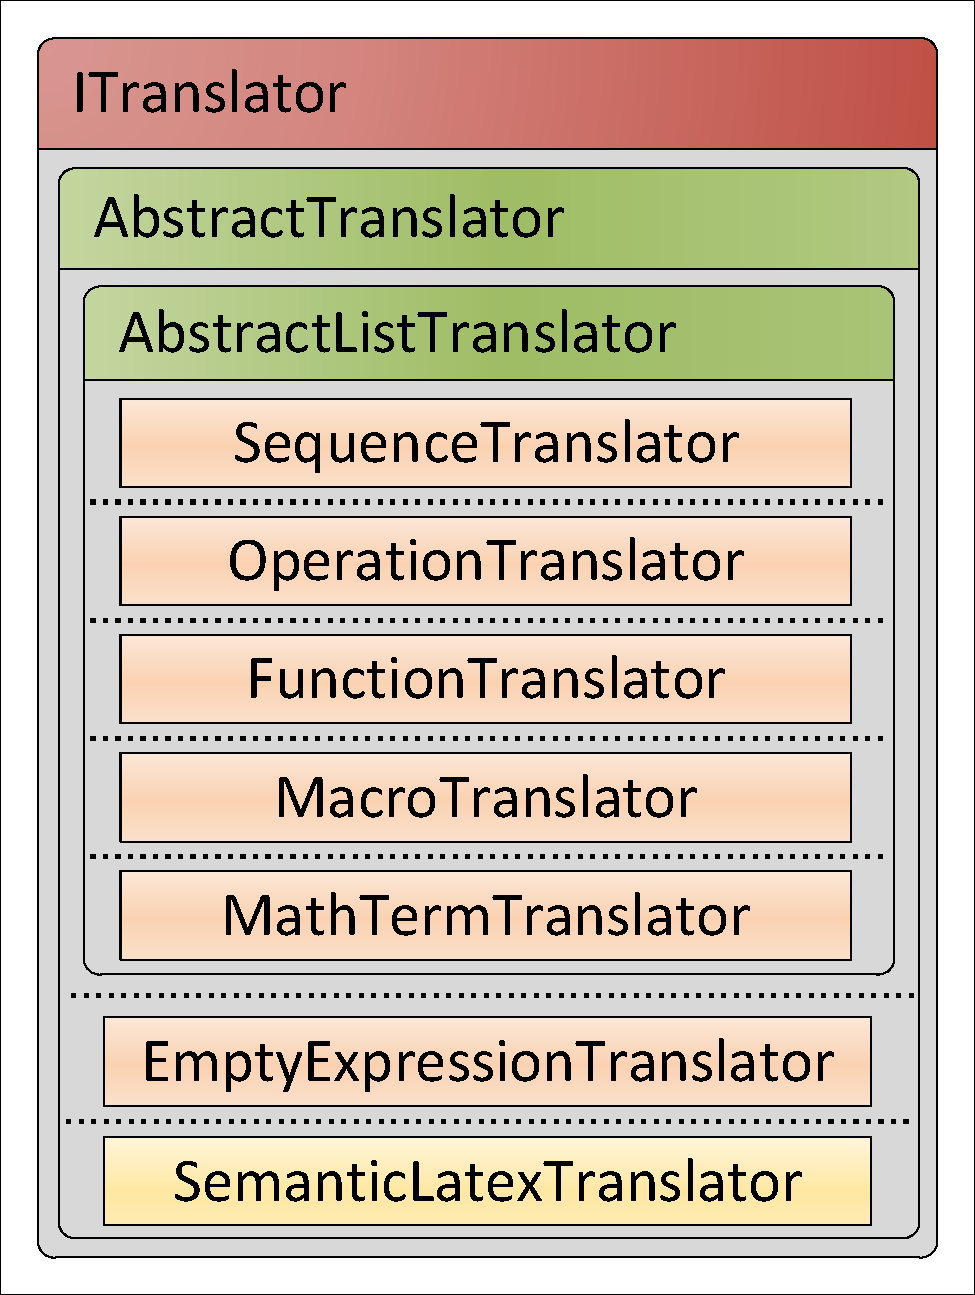
\includegraphics[clip, trim=0.1cm 0.1cm 0.1cm 0.1cm, scale=0.4]{ForwardTranslator.pdf}
	\caption{A scheme of the forward translator and its specialized subtranslators.}
	\label{fig:ForwardDel}
	\vspace{-25pt}
\end{wrapfigure}

Algorithm~\ref{alg:translation} is a simplified version of the translator process. The main progress happens in \cref{line:transLeaf,line:transSeq}. There are several cases what $r$ can be. Table~\ref{tab:allTypesTable} on page \pageref{tab:allTypesTable} gives an overview of all different types in a \gls{mlp-pt}. A more detailed explanation of the types can be found in~\cite{POM-Tagger}. 

The \gls{bnf} grammar defines some basic grammatical rules for generic \LaTeX{} macros, such as for \verb|\frac|, \verb|\sqrt|. Therefore, there is a hierarchical structure for those symbols, similar to the structure in expression trees. As already mentioned, some of these types can be translated directly, such as Greek letters, while others are more complex, such as semantic \LaTeX{} macros. Therefore, the translators delegates the translation to specialized subtranslators. This delegation process is implemented in \cref{line:transLeaf,line:transSeq} of algorithm~\ref{alg:translation}.

Figure~\ref{fig:ForwardDel} is a scheme of the forward translator and its subtranslators. The entry point for each translation process of the program is the \verb|SemanticLatexTranslator|. It delegates the translations for the expression through the \verb|AbstractTranslator| to the other subtranslators. The \verb|AbstractTranslator| is the interface of all other translators and coordinates the translation process by delegating translations for specific nodes to specialized classes. For example, the \verb|MacroTranslator| only translates semantic \LaTeX{} macros. The \verb|EmptyExpressionTranslator| is used to delegate the so called \textit{empty expressions} to other classes. An \textit{empty expression} is a node with children, but without a symbol itself, such as \textit{sequences} and \textit{balanced expressions}.

\subsubsection{Subtranslators}
The most interesting translators are the \verb|MacroTranslator| (translating semantic \LaTeX{} macros) and the \verb|SequenceTranslator| (translating all kinds of \textit{sequences}).

The \verb|SequenceTranslator| translates the \textit{sequence} and \textit{balanced expressions} in the \gls{mlp-pt}. If a node $n$ is a leaf and the represented symbol an open bracket (parentheses, square brackets and so on) the following nodes are also taken as a \textit{sequence}. Hence, combined with the recursive translation approach, the \verb|SequenceTranslator| also checks balances of parentheses in expressions. An expression such as '$(a]$' is producing a mismatched parentheses error. On the other hand, this is a problem for interval expressions such as '$[a,b)$'. In the current version, the program cannot distinguish between mismatched parentheses and an half-opened, half-closed interval. Whether an expression is an interval or another expression is difficult to decide and can depend on the context. In addition, the parenthesis checker could simply be deactivated to allow mismatched parentheses in an expression. But this functionality is not implemented yet.

Another problem that the \verb|SequenceTranslator| solves is the position of multiplication signs in an expression. There are a couple of obvious choices to translate multiplication signs. For example, using \verb|\cdot| or \verb|\idot| will be obviously translated as a multiplication symbol. However, \verb|\idot| is fairly new and therefore not frequently used yet. Furthermore, the most common symbol for multiplications is still the white space or none symbol at all, as explained above. Consider the simple expression $2n\pi$. The \gls{mlp-pt} generates a sequence node with three children, namely $2$, $n$ and $\pi$. This sequence should be interpreted as a multiplication of the three elements. Therefore, the \verb|SequenceTranslator| checks the types of the current and next nodes in the tree to decide if there should be a multiplication symbol or not. For example, if the current or next node is an operator, a relation symbol or an ellipsis there will be no multiplication symbol added. However, this approach implies an important property. The translator interprets all sequences of nodes as multiplications as long as it is not defined otherwise. This potentially produces strange effects. Consider an expression such as $f(x)$. Translate this to \Maple{} will be \verb|f*(x)|. But we do not consider this translation to be wrong, because there is a semantic macro to represent functions. In this case, the user should use \verb|\f{f}@{x}| instead of \verb|f(x)|.

Besides the translation of sequences, the translation process of the \Macro s can be complex too; not only because of the structure of the \gls{mlp-pt}, but also because of the complex definition of the semantic macros. As explained in \ref{subsec:macros}, they can contain optional parameters, exponents are allowed before and after the arguments and the number of $@$ symbols varies. All these different cases will be solved by the \verb|MacroTranslator|. 

Algorithm~\ref{alg:macro-translation} is the translation function of the \verb|MacroTranslator| without error handling. It analyzes the next element right after the macro first. As mentioned, this can be one of the following:
\begin{itemize}
\item an exponent such as '\verb|^2|'.
\item an optional parameter in square brackets.
\item a parameter in curly brackets (a \textit{sequence} node in the \gls{mlp-pt}) if none of the above.
\item an $@$ symbols if none of the above.
\item a variable in curly brackets (a \textit{sequence} node) if none of the above.
\end{itemize}
\begin{algorithm}[!ht]
\caption{The translate function of the MacroTranslator. This code ignores error handling.}\label{alg:macro-translation}
	\begin{algorithmic}[1]
	\Require 
		\Statex \textit{macro} - node of the semantic macro. 
		\Statex \textit{args} - list of the following siblings of \textit{macro}. 
		\Statex \textit{lexicon} - lexicon file
	\Ensure 
		\Statex Translated semantic macro.
	
	\Procedure{translate\_macro}{\textit{macro}, \textit{args}, \textit{lexicon}}
	\State \textit{info} = \textit{lexicon}.getInfo(\textit{macro});
	\State \textit{argList} = new List(); \Comment{create a sorted list for the translated arguments.}
	\State \textit{next} = \textit{args}.getNextElement();
	\If{\textit{next} is caret}\label{line:next_caret}
		\State \textit{power} = translateCaret(\textit{next});
		\State \textit{next} = \textit{args}.getNextElement();
	\EndIf
	
	\While{\textit{next} is $[$}\label{line:next_optional} \Comment{square brackets indicate optional arguments.}
		\State \textit{optional} = {\scriptsize TRANSLATE\_UNTIL\_CLOSED\_BRACKET}(\textit{args});
		\State \textit{argList}.add(\textit{optional});
		\State \textit{next} = \textit{args}.getNextElement();
	\EndWhile
	
	\State \textit{argList}.add( {\scriptsize TRANSLATE\_PARAMETERS}(\textit{args}, \textit{info}) ); \label{line:trans_paras}
	\State {\scriptsize SKIP\_AT\_SIGNS}( \textit{args}, \textit{info} ); \label{line:skip_ats}
	\State \textit{argList}.add( {\scriptsize TRANSLATE\_VARIABLES}(\textit{args}, \textit{info}) ); \label{line:trans_vars}
	
	\State \textit{pattern} = \textit{info}.getTranslationPattern();
	\State \textit{translatedMacro} = \textit{pattern}.fillPlaceHolders(\textit{argList});
	\If{\textit{power} is not \NULL}
		\State \textit{translatedMacro}.add(\textit{power});
	\EndIf
	\State \Return\ \textit{translatedMacro};
	\EndProcedure
	\end{algorithmic}
\end{algorithm}

An exponent will be translated and shifted to the end of the translated semantic macro, since it is more common to write the exponent after the arguments of a function in \gls{cas}. Therefore, the function translates and stores the exponent in line~\ref{line:next_caret}. One could ask what happens when there is an exponent given before and after the arguments. The \verb|MacroTranslator| only translates the following siblings until each argument is translated. The first exponent will be shifted to the end. If right after the translated macro (with all arguments) follows another exponent, we interpret it as another exponent for the whole previous expression. In that case, it would be the macro with the first translated exponent. Table~\ref{tab:multi-expo} shows an example for the trigonometric cosine function with multiple exponents. 
\begin{table}[ht]
\centering
\begin{tabular}{lc}
\hline
Displayed As & \rule{0pt}{0.9\normalbaselineskip} $\cos^2(x)^2$ \\
Semantic \LaTeX & \verb|\cos^2@{x}^2| \\
Translated \Maple{} Expression & \verb|((cos(x))^(2))^2|\\
\hline
\end{tabular}
\caption{A trigonometric cosine function example with exponents before and after the argument.}
\label{tab:multi-expo}
\end{table}

As you can see, the input expression in semantic \LaTeX{} is interpreted as~\eqref{eq:multi-expo}.
\begin{equation}\label{eq:multi-expo}
\left( \cos(x)^2 \right)^2
\end{equation}

An open square bracket right after the semantic macro (after the exponent respectively) is an optional parameter. Since expressions in square brackets are not considered to be a \textit{sequence} in the \gls{mlp-pt}, the optional parameter is not grouped in a single node. Therefore, every node after the opening square bracket forms an expression for just one optional parameter until the algorithm reaches the closing square bracket. Such expressions in square brackets will be also translated by the \verb|SequenceTranslator| as described above. A semantic macro could have multiple optional parameters. Therefore, the function translates all optional parameters and stores them in line~\ref{line:next_optional}.

The \cref{line:trans_paras,line:skip_ats,line:trans_vars} translates the parameters and variables. The $@$ symbols will be skipped. Nevertheless, the current program has an error handling implemented in \cref{line:skip_ats} if the maximum number of $@$ symbols is exceeded. In the following lines, the function takes the translation pattern from the lexicon and removes each placeholder by the corresponding argument. In addition, if there is an exponent right after the semantic macro, it will be attached to the translated semantic macro (see table~\ref{tab:multi-expo}). The parameters and variables are always grouped by curly brackets in \textit{sequence}-nodes in the \gls{mlp-pt}. Therefore, every argument after the optional parameters and potential exponent cannot be longer than one node in the \gls{mlp-pt}.

\subsubsection{Handle Ambiguities}\label{subsec:ambiguities}
Our semantic \LaTeX{} expressions are not full semantic with respect to possible ambiguities in the expression. We already mentioned some techniques to solve ambiguities in semantic \LaTeX{} expressions, for example how to handle double factorials. In table~\ref{tab:amb-latex} are four examples of ambiguous expressions. \LaTeX{} implemented the rules that the superscript or subscript is only one symbol (or a balanced expression in curly brackets). Therefore, each of these input expressions are not ambiguous in \LaTeX. Since we talking about the forward translation, we should follow the rules of \LaTeX{} to interpret ambiguous expressions.

\begin{table}[ht]
\centering
\begin{tabular}{cc}
	\hline
	Ambiguous Input & \LaTeX{} Output\\
	\hline
	\verb|n^m!| & $n^m!$\\
	\verb|a^bc^d| & $a^bc^d$\\
	\verb|x^y^z| & Double superscript error\\
	\verb|x_y_z| & Double subscript error\\
	\hline
\end{tabular}
\caption{Ambiguous \LaTeX{} expressions and how \LaTeX{} displays them.}
\label{tab:amb-latex}
\end{table}

Another more questionable translation decision are alphanumerical expressions. As explained in table~\ref{tab:allTypesTable}, the \gls{mlp} handles strings of letters and numbers differently, depending on the order of the symbols. The reason is, that an expression such as '$4b$' is usually considered to be a multiplication of $4$ and '$b$', while '$b4$' looks like indexing '$b$' by $4$. While the first example produces two nodes, namely $4$ and '$b$', the second example '$b4$' produces just a single alphanumerical node in the \gls{mlp-pt}. The first expression would be translated as a multiplication of $4$ and '$b$'. Because '$4b$' looks like '$4 \cdot b$' and the multiplication is commutative, we would assume that '$4b$' and '$b4$' are equivalent. This is one reason why we interpret such alphanumerical expressions as multiplications of the symbols. On the other hand, an expression such as '$energy$', would be an alphanumerical node as well and could be interpreted as a single variable named 'energy'. In that case, someone could wonder why the variable '$energy$' was translated as '$e \cdot n \cdot e \cdot r \cdot g \cdot y$'. While in physics or engineering variables possibly appear with longer names, such as the 'energy' example, it is more common to use single symbols for variables in mathematics~\cite{Notation:History}. Therefore, we interpret such alphanumerical expressions as multiplications of variables rather than one variable with an alphanumerical name.

Another, more elegant way to solve this problem would be to use the newly created semantic macro \verb|\idot| (see subsection~\ref{subsec:semanticVSmacro}) to define an invisible multiplication symbol. However, because \verb|\idot| is such a new semantic macro, it is not used in the \gls{dlmf} or \gls{drmf} quite often yet. Therefore, our program still interprets alphanumerical expressions as multiplications.

Other ambiguities can appear, when the input expression contains a symbol, which is typically used to represent a specific mathematical object, but the user did not use the semantic macro to represent it. For example, the input expressions '$3i$' contains an '$i$', which is usually associated with the imaginary unit. Since there is a semantic macro for the imaginary unit, namely \verb|\iunit|, we do not translate the letter to the imaginary symbol in \Maple{} and use the identity translation instead. Furthermore, we inform the user about the potential misusage of \verb|i| (see~\ref{subsec:add-info}).

In general the translator is drafted to solve ambiguous expressions or automatically find a workaround to disambiguate the expression. Only if there is no way to solve the ambiguity with the defined rules, the translation process stops.

\subsection{Translated Expression Objects}\label{subsec:translated-expr}
\glsreset{teo}
\begin{wrapfigure}{r}{0.5\textwidth}
	\vspace{-20pt}
	\centering
	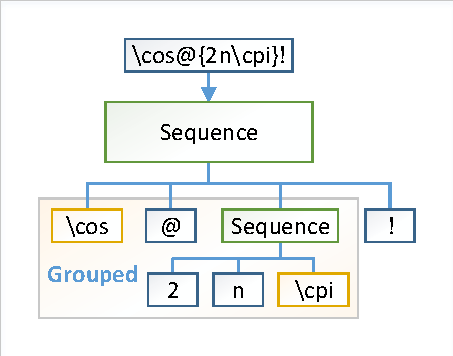
\includegraphics[clip, trim=0.2cm 0.2cm 0.2cm 0.2cm, scale=1]{SyntaxTreeGroup.pdf}
	\caption{The MLP-PT for '$\cos(2n\pi)!$' and the grouped argument of the factorial function.}
	\label{fig:syntax-group}
	\vspace{-15pt}
\end{wrapfigure}

It is sometimes necessary to provide access to already translated symbols or subexpressions. A typical example is the (double) factorial function, where the argument was translated before the function was registered by the translator (postfix notation). To realize this, the \gls{teo} is implemented. It is mainly a list object of translated expressions. It also groups subexpressions when it becomes clear that multiple symbols belong together. This typically happens when something is wrapped in parentheses but also when a function is completely translated.   

Figure~\ref{fig:syntax-group} shows an example for the expression '$\cos(2n\pi)!$'. If we just analyze the \gls{mlp-pt}, the previous node of the exclamation mark (which indicates the factorial function) is the sequence. Now it could be possible to misinterpret the sequence as the argument of the factorial function. But the translator will first translate the cosine function, which has one argument. In that case the argument is the sequence node. Once the cosine function has been completely translated (which means the whole argument has been translated as well) the \gls{teo} groups the translated cosine and the sequence. Therefore, when the translator reaches the exclamation mark and asks for the last translated object in the list, it is not the translated sequence but the whole cosine function.

Table~\ref{tab:teo-list} shows some examples of the \gls{teo} list after the translation process was finished. Note that a translation of '$a+b$' contains three translated objects, while '$(a+b)$' contains just one.

\begin{table}[ht]
\centering
\begin{tabular}{cc}
	\hline
	Input Expression & TEO List\\
	\hline
	$a+b$ & \verb|[a, +, b]|\\
	$(a+b)$ & \verb|[(a+b)]|\\
	$\frac{a}{b}-2$ & \verb|[(a)/(b), -, 2]|\\
	\hline
\end{tabular}
\caption{How the TEO-list groups subexpressions.}
\label{tab:teo-list}
\end{table}

\subsubsection{Local \& Global Translated Expressions}
During the translation process multiple local \gls{teo} are created by the subtranslators. Besides the local \gls{teo} there is just one global \gls{teo}. The reason to create local objects is originally motivated by the recursive structure of the translator. A subtranslator should only handle the current subexpression. However, the global \gls{teo} becomes necessary because of the functions in postfix notation such as the factorial function. For example, when a subtranslator tries to translate the exclamation mark as the factorial function, the local \gls{teo} is empty, because the argument of the function has been previously translated by another subtranslator and stored in another local \gls{teo}. Therefore, we implement a global \gls{teo}, which contains all of the previous translated subexpressions in each state of the translation process. With this implementation the local \gls{teo} becomes more and more obsolete. In the current version, the program stores redundant translated expressions. For debugging reasons, a translation process still handles multiple local and one global \gls{teo}. Starting the forward translation with the flag \verb|--debug| (for the debugging mode) shows the elements of the global \gls{teo} after the translation has been finished.

\subsection{Additional Information}\label{subsec:add-info}
As already mentioned, a translation is not always straight forward. In those cases, the user should get informed about the translation and the reason for it. Consider the translation
\begin{equation}\label{eq:i-trans}
\verb|3i| \overset{\langMaple}{\mapsto} \verb|3*i|,
\end{equation}
Since the imaginary unit in \Maple{} is associated with '\raw{I}' instead of '\raw{i}', a user might be confused by~\ref{eq:i-trans}. Therefore, we created the \texttt{InformationLogger} class to organize further information about the translation process. In the case of '\raw{i}', the user is informed about the semantic macro \verb|\iunit| and the potential misusage of '\raw{i}'.

Essentially, the \raw{InformationLogger} provides further information about a translation process. This information is defined in the lexicon files. Consider the example of the arccotangent function, which is defined with a different branch cut in \gls{dlmf} and in \Maple. As already mentioned, we provide alternative translation patterns to solve these problems. These alternative translations, explanations, branch cuts, domains etc. will be automatically stored in the \raw{InformationLogger} when an expression contains a mathematical object with further information.